\renewcommand{\familydefault}{\sfdefault}
\documentclass{scrartcl}
\usepackage{amsmath}
\usepackage[utf8]{inputenc}
\usepackage{natbib}
\usepackage{graphicx}
\usepackage{tikz}
\usepackage{float}

\begin{document}
\title{Saving Honey}
\author{}
\date{December 2020}
\setlength\parindent{0pt}


\maketitle

\section{23/10/2021-Modelling motion of single drop on cylinder}
\begin{figure}[h]
    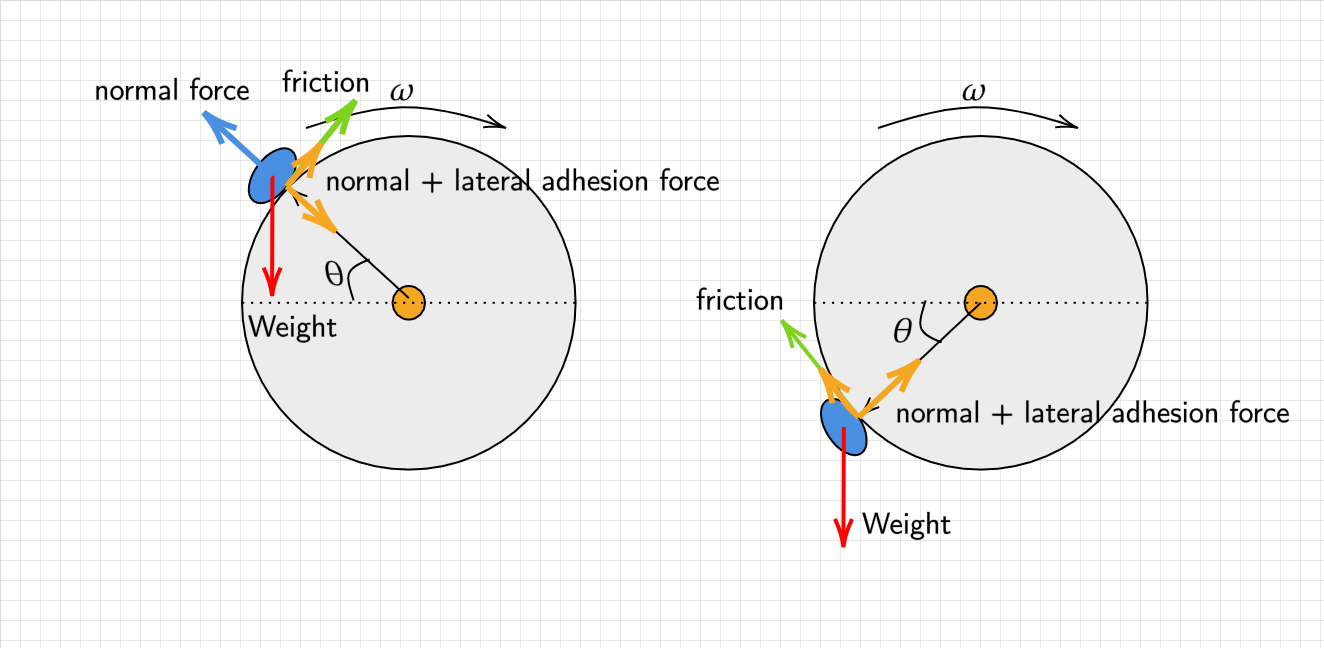
\includegraphics[width=\textwidth]{diagram-20211030.png}
\end{figure}

From online: Adhesion force characterizes the force that is required to detach a liquid droplet from a surface that it contacts. It provides a way to quantify the attractive interaction between liquid and solid.

It is impossible for the droplet to remain stationary at the top and bottom points of the rotating cylinder (there is nothing to balance out friction)

\subsection{condition for drop to remain stationary on the rotating cylinder}
\begin{itemize}
    \item net tangential force $=0$
    \item drop must remain in contact with the surface of the cylinder
\end{itemize}

Adhesion force is quite complicated so let's just call it $F_{lat}$ and $F_{norm}$ for now i guess.

\subsection{balancing tangential forces}
\begin{equation}
    mg\cos\theta=\mu N + F_{lat}
\end{equation}

\subsection{balancing radial forces}
For the first case (left) where the drop is resting on the surface
\begin{equation}
    F_{norm}-N= mr\omega ^2 
\end{equation}
For the second case (right )where the drop is hanging from the surface 
\begin{equation}
    F_{norm}= mr\omega ^2 
\end{equation}

\subsection{more about adhesion force}
\begin{figure}[h]
    \centering
    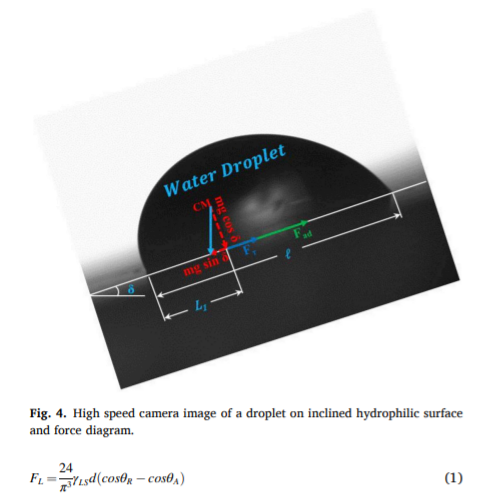
\includegraphics[scale=1.1]{adhesion equation from research paper.png}
\end{figure}

$\theta_A$ and $\theta_R$ are the advancing and receding angle respectively. 

\begin{figure}
    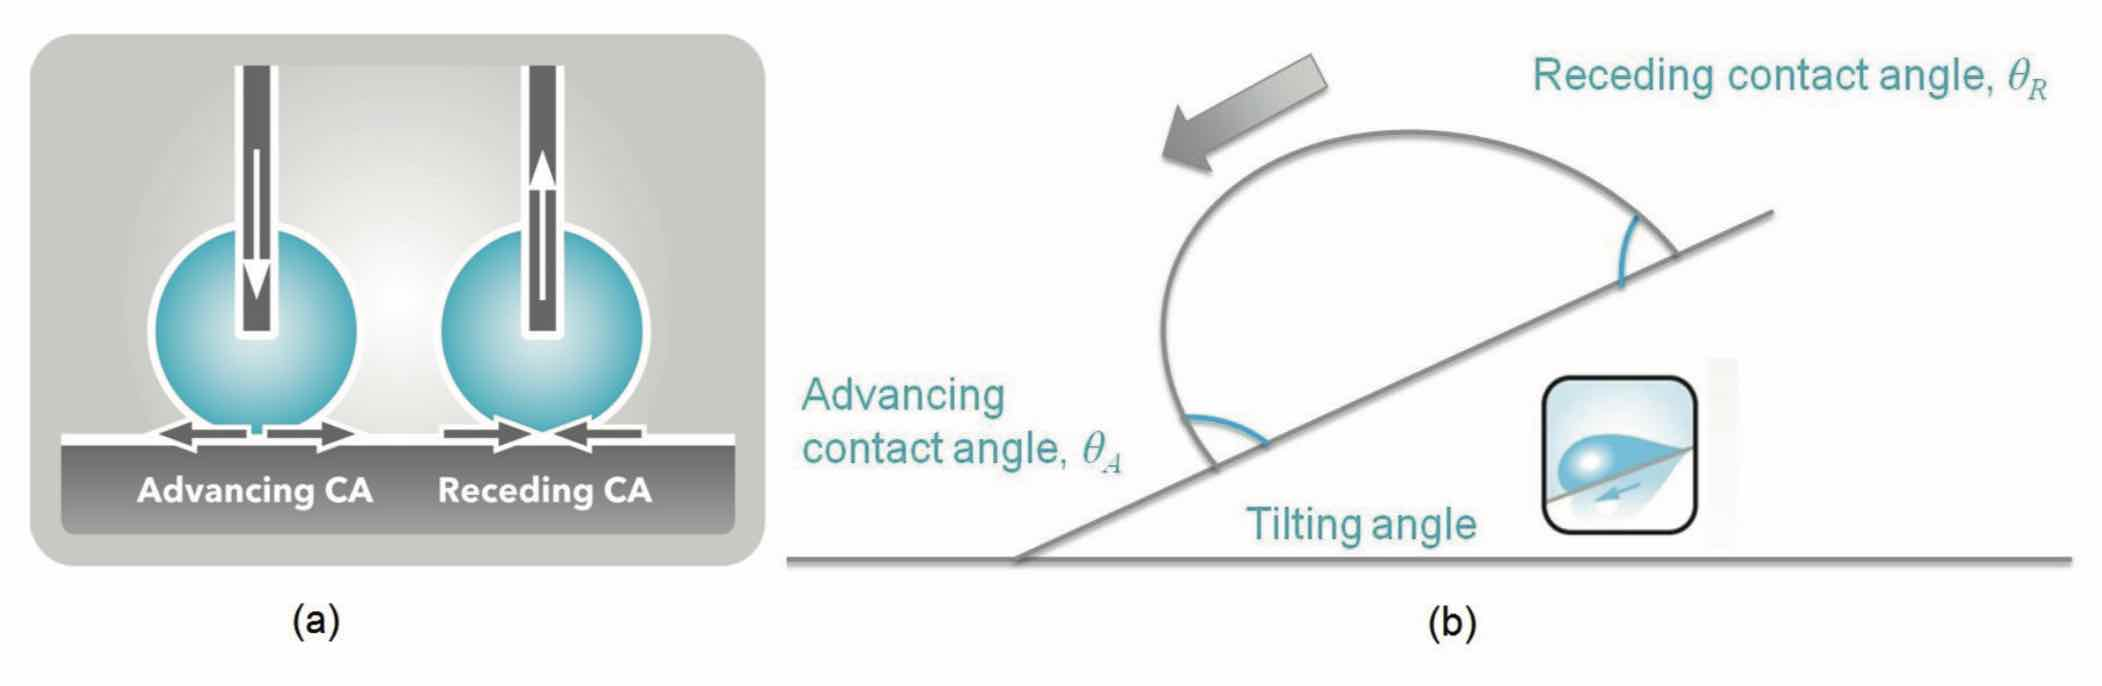
\includegraphics[width=\linewidth]{Dynamic-Contact-Angle-Measurement.jpg}
\end{figure}

As tilting angle increases, the advancing contact angle ($\theta_A$) would decrease, and the receding angle ($\theta_R$) would increase. so the value of lateral adhesion force would 

\subsection{Oscillation?}
\begin{figure}[h]
    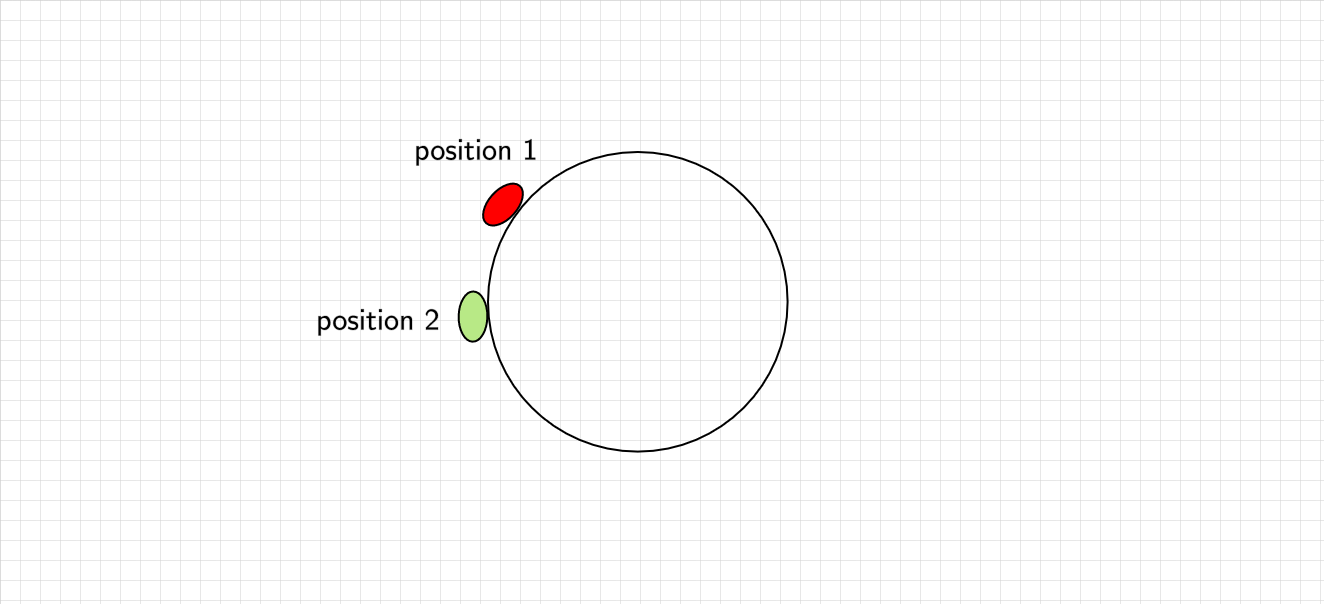
\includegraphics[width=\linewidth]{diagram-20211030 (1).png}
\end{figure}
    
If the drop is perturbed by dk what then it moves from position 1 to position 2, the advancing contact angle would increase and receding contact angle would decrease. 

\begin{figure}[H]
    \centering
    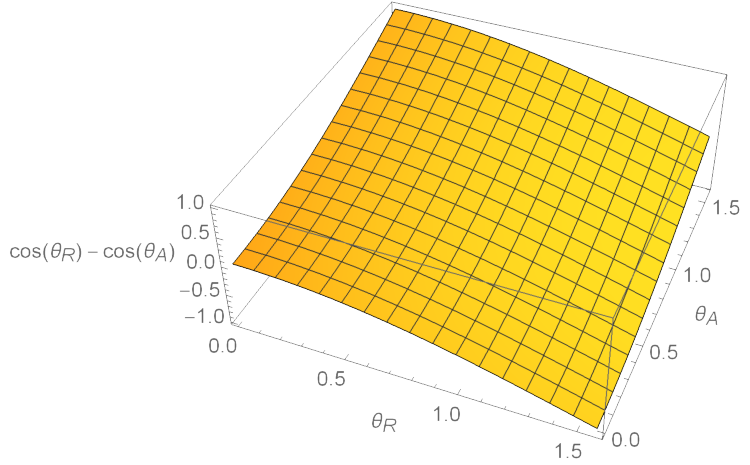
\includegraphics[scale=1]{cos(x)-cos(y).pdf}
\end{figure}
Shown in this figure, $\cos \theta_R-\cos \theta_A$ increases as $\theta_A$ increases and $\theta_R$ decreases. Lateral adhesion force increases. 
\begin{equation}
    \mu N + F_{lat}-mg\cos\theta> 0
\end{equation}

\section{04/11/2021-modelling height of fluid as a function of angle}

\end{document}

